\section{Empirical Results}
\label{sec:results}

We report our empirical findings structured around the four research questions, validating all numerical claims against the frozen canonical prediction records.

\subsection{RQ1: Prediction Disagreement and Directional Transitions}
When evaluating identical claim-evidence pairs across machine-translated English ($e_{\text{trans}}$) and original Hindi ($e_{\text{orig}}$), verifier predictions diverge substantially. Across the $N=163$ test instances, the verifier agrees on only 59 instances (36.20\%; 95\% CI: [29.22\%, 43.81\%]) and disagrees on \textbf{104 instances (63.80\%; 95\% CI: [56.19\%, 70.78\%])}.

\begin{table}[t]
\centering
\small
\caption{Empirical $3 \times 3$ directional transition matrix on the test set ($N=163$), cross-tabulating predictions between machine-translated English evidence (rows) and original Hindi evidence (columns). Over 63.8\% of instances flip predictions across language representations.}
\label{tab:transition_matrix}
\begin{tabular}{lcccc}
\toprule
\textbf{Translated Prediction} & \multicolumn{3}{c}{\textbf{Original Hindi Prediction}} & \textbf{Row Total} \\
\cmidrule(lr){2-4}
($e_{\text{trans}}$) & \textsc{Contradicted} & \textsc{Insufficient} & \textsc{Supported} & ($N_{\text{trans}}$) \\
\midrule
\textsc{Contradicted} & 21 (12.9\%) & 5 (3.1\%) & 18 (11.0\%) & 44 (27.0\%) \\
\textsc{Insufficient} & 23 (14.1\%) & 14 (8.6\%) & 18 (11.0\%) & 55 (33.7\%) \\
\textsc{Supported}    & 31 (19.0\%) & 9 (5.5\%) & 24 (14.7\%) & 64 (39.3\%) \\
\midrule
\textbf{Column Total} ($N_{\text{orig}}$) & \textbf{75 (46.0\%)} & \textbf{28 (17.2\%)} & \textbf{60 (36.8\%)} & \textbf{163 (100.0\%)} \\
\bottomrule
\end{tabular}
\end{table}


Table~\ref{tab:transition_matrix} presents the complete $3 \times 3$ directional transition matrix. The rows represent predictions under machine-translated evidence ($\hat{y}_{\text{nc}}$), while columns represent predictions under original Hindi evidence ($\hat{y}_{\text{dm}}$). Figure~\ref{fig:fig5_heatmap} visualizes these transitions as a normalized transition heatmap.

\begin{figure}[t]
\centering
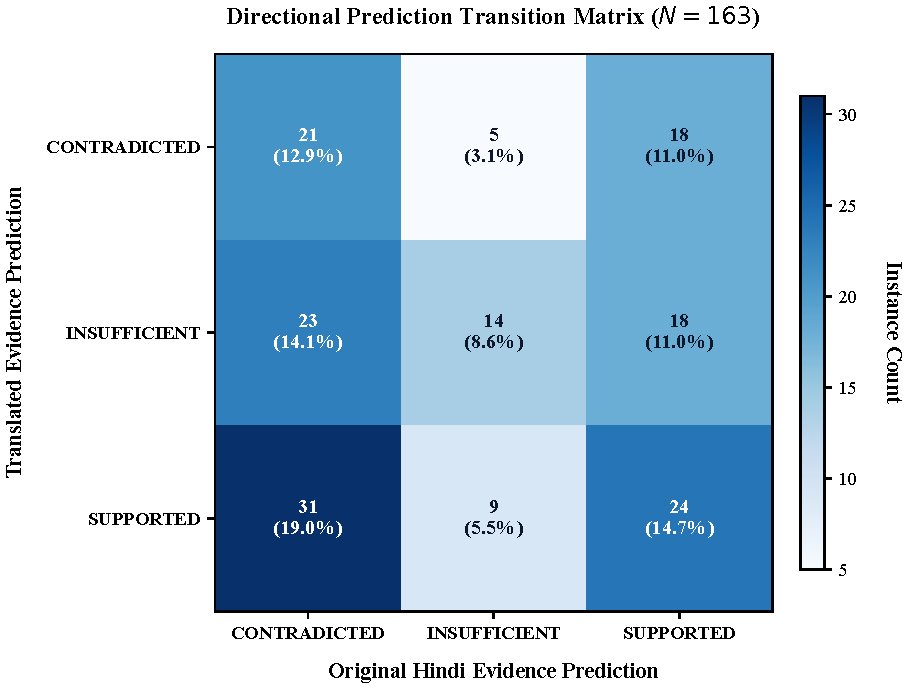
\includegraphics[width=\columnwidth]{figures/final/fig5_transition_heatmap.pdf}
\caption{Directional prediction transition heatmap ($N=163$). Cell values indicate raw counts and row-conditional percentages (\%) of original Hindi predictions given translated English predictions.}
\label{fig:fig5_heatmap}
\end{figure}

The transition matrix reveals pronounced asymmetric error dynamics:
\begin{enumerate}
    \item \textbf{False Support to Refutation Flips:} Of the 64 instances predicted as \textsc{Supported} under translated English evidence, \textbf{31 instances (48.44\%; 95\% CI: [36.56\%, 60.52\%])} flip to \textsc{Contradicted} when evaluated on original Hindi evidence. Because the test set contains zero gold \textsc{Supported} instances, these 31 cases represent instances where translation shift induced spurious entailment that original evidence successfully refuted.
    \item \textbf{Decisive Refutation to False Support Flips:} Conversely, of the 44 instances predicted as \textsc{Contradicted} under translated evidence, \textbf{18 instances (40.91\%; 95\% CI: [27.70\%, 55.59\%])} flip to \textsc{Supported} under original Hindi evidence.
    \item \textbf{Uncertainty Transitions:} Of the 55 instances predicted as \textsc{Insufficient\_Evidence} under translated evidence, 23 (41.82\%) resolve to \textsc{Contradicted} and 18 (32.73\%) flip to \textsc{Supported} under original Hindi evidence. Only 14 instances (25.45\%) remain stably classified as insufficient evidence across both representations.
\end{enumerate}

\subsection{RQ2: Benchmark Performance Across Verification Conditions}
Table~\ref{tab:main_results} compares the performance of the four verification conditions alongside majority and random baselines on the $N=163$ test partition.

\begin{table*}[t]
\centering
\small
\caption{Benchmark performance across verification conditions on the X-Fact Hindi test set ($N=163$). 95\% confidence intervals for accuracy are computed via Wilson score intervals. Observed 2-class Macro-F1 evaluates \textsc{Contradicted} and \textsc{Insufficient\_Evidence}; nominal 3-class Macro-F1 includes the absent \textsc{Supported} class ($F_{1,\text{SUP}}=0.0$). The cascade threshold $\tau^*=0.650$ was tuned strictly on development data.}
\label{tab:main_results}
\resizebox{\textwidth}{!}{%
\begin{tabular}{lcccccc}
\toprule
\textbf{Verification Pipeline / Baseline} & \textbf{Coverage} & \textbf{Accuracy [95\% CI]} & \textbf{Macro-F1 (2-cl)} & \textbf{Macro-F1 (3-cl)} & \textbf{Mean Latency} & \textbf{Compute Ratio} \\
\midrule
No-Check (Translated English Only) & 0.0\% (0/163) & 0.2822 [0.2147, 0.3558] & 0.3018 & 0.2012 & 3,650.4 ms & $1.0\times$ \\
Direct Multilingual (Original Hindi Only) & 100.0\% (163/163) & \textbf{0.4294} [0.3557, 0.5092] & \textbf{0.3700} & \textbf{0.2467} & 11,295.6 ms & $3.1\times$ \\
Always-Check (Dual Consensus Posterior Avg) & 100.0\% (163/163) & 0.3681 [0.2945, 0.4417] & 0.3657 & 0.2438 & 14,945.9 ms & $4.1\times$ \\
Selective-Check ($\tau^*=0.650$, Hard Route) & 8.0\% (13/163) & 0.2822 [0.2147, 0.3558] & 0.2950 & 0.1967 & 4,613.8 ms & $1.3\times$ \\
\midrule
\multicolumn{7}{l}{\emph{Diagnostic Controls and Baseline Benchmarks}} \\
Ablation: Triggered Posterior Averaging & 8.0\% (13/163) & 0.2699 [0.2025, 0.3436] & 0.2854 & 0.1903 & 4,613.8 ms & $1.3\times$ \\
Ablation: Uncertainty-Only Fallback & 8.0\% (13/163) & 0.2822 [0.2147, 0.3558] & 0.3018 & 0.2012 & 4,613.8 ms & $1.3\times$ \\
Ablation: Numeral-Only Fallback & 96.3\% (157/163) & 0.4479 [0.3742, 0.5276] & 0.3794 & 0.2529 & 14,751.3 ms & $4.0\times$ \\
Random Routing Control (100 Seeds, Cov=8.0\%) & 8.0\% (13/163) & 0.2924 [0.2638, 0.3190] & 0.3082 & 0.2054 & 4,613.8 ms & $1.3\times$ \\
Majority Baseline (Always \textsc{Contradicted}) & 0.0\% (0/163) & 0.8712 [0.8116, 0.9139] & 0.4656 & 0.3104 & --- & --- \\
Oracle Upper Bound (Non-Deployable Upper Bound) & 100.0\% (163/163) & 0.5951 [0.5215, 0.6687] & 0.5200 & 0.3467 & 14,945.9 ms & --- \\
\bottomrule
\end{tabular}%
}
\end{table*}


\paragraph{Direct Multilingual Superiority.}
Evaluating original Hindi evidence directly (\emph{Direct Multilingual}) achieves an overall accuracy of \textbf{42.94\% (70/163; 95\% CI: [35.58\%, 50.65\%])}, compared to \textbf{28.22\% (46/163; 95\% CI: [21.84\%, 35.62\%])} for the translated-evidence \emph{No-Check} baseline---an absolute accuracy advantage of $+14.72\%$. 

Direct Multilingual verification achieves substantial gains on the dominant majority class (\textsc{Contradicted}), elevating recall from 14.79\% (21/142) under translated evidence to 39.44\% (56/142) under original Hindi, with precision increasing from 47.73\% to 74.67\%. As visualized in Figure~\ref{fig:fig3_comparison}, Direct Multilingual demonstrates superior class-balanced precision-recall trade-offs across non-empty classes.

\begin{figure}[t]
\centering
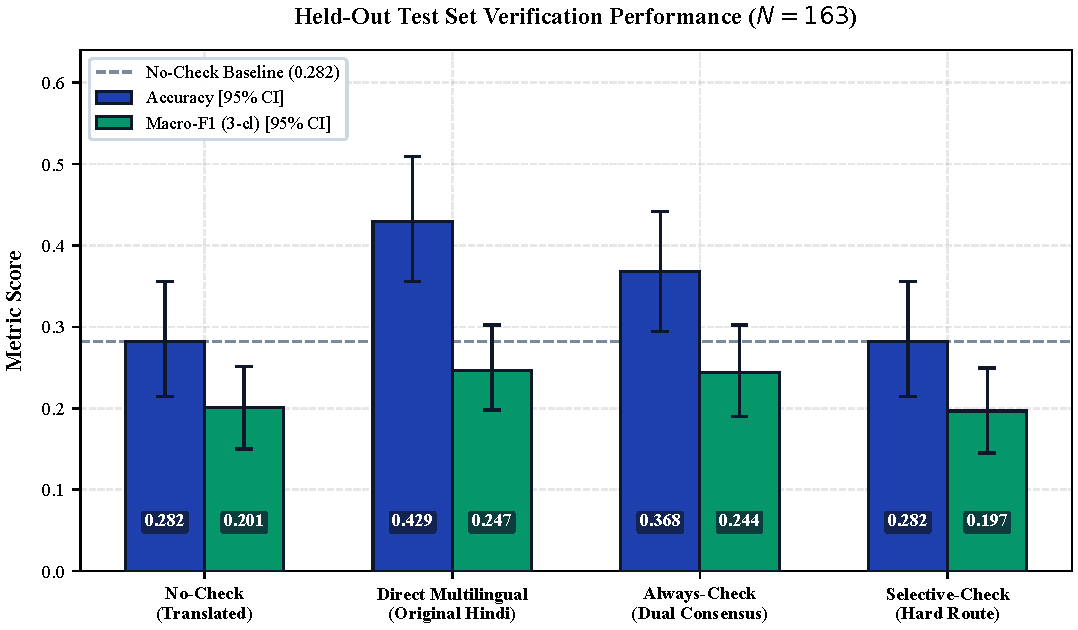
\includegraphics[width=\columnwidth]{figures/final/fig3_condition_comparison.pdf}
\caption{System performance comparison across accuracy, 3-class Macro-F1, and 2-class Macro-F1 on the $N=163$ test split with 95\% Wilson score confidence intervals.}
\label{fig:fig3_comparison}
\end{figure}

\subsection{RQ3: Paired Statistical Comparisons and Metric Discordance}
Table~\ref{tab:statistical_tests} reports the formal paired statistical hypothesis tests comparing Direct Multilingual against No-Check, Selective-Check, and Always-Check.

\begin{table*}[t]
\centering
\small
\caption{Paired statistical significance tests across verification conditions on the test set ($N=163$). McNemar tests evaluate paired marginal accuracy on discordant pairs ($b, c$) with continuity correction and exact binomial $p$-values. Permutation tests evaluate the null distribution of paired Macro-F1 deltas ($B=5,000$ resamples, seed 42). Benjamini-Hochberg False Discovery Rate (FDR) adjustments ($q$-values) are reported for multiple-testing control across the comparison family.}
\label{tab:statistical_tests}
\resizebox{\textwidth}{!}{%
\begin{tabular}{lcccccc}
\toprule
\textbf{Pairwise Comparison Condition} & \textbf{Discordant ($b, c$)} & \textbf{McNemar $\chi^2$} & \textbf{Exact $p_{\text{raw}}$} & \textbf{FDR $p_{\text{adj}}$} & $\Delta$\textbf{Macro-F1 (3cl)} & \textbf{Perm. $p_{\text{raw}}$} \\
\midrule
No-Check vs. Direct Multilingual & $b=27, c=51$ ($n=78$) & 6.7821 & \textbf{0.008772} & \textbf{0.0175} & $-0.0455$ & 0.18980 \\
Selective-Check vs. Direct Multilingual & $b=23, c=47$ ($n=70$) & 7.5571 & \textbf{0.005583} & \textbf{0.0149} & $-0.0500$ & 0.11800 \\
Selective-Check vs. Always-Check & $b=9, c=23$ ($n=32$) & 5.2812 & \textbf{0.02006} & \textbf{0.0401} & $-0.0471$ & \textbf{0.01960} \\
Selective-Check vs. No-Check & $b=4, c=4$ ($n=8$) & 0.1250 & 1.0000 & 1.0000 & $-0.0045$ & 0.75720 \\
Selective-Check vs. Random Control (100 Seeds) & $b=4, c=9$ (avg) & 1.2308 & 0.26685 & 0.4270 & $-0.0208$ & 0.16500 \\
Selective-Check vs. Numeral-Only Routing & $b=20, c=47$ ($n=67$) & 10.0896 & \textbf{0.00131} & \textbf{0.0052} & $-0.0563$ & 0.07440 \\
\bottomrule
\end{tabular}%
}
\end{table*}


\paragraph{McNemar Correctness Significance.}
Under McNemar's paired test for marginal binary correctness:
\begin{itemize}
    \item \textbf{No-Check vs. Direct Multilingual:} The systems disagree on $n = 78$ discordant instances. Direct Multilingual is correct while No-Check is incorrect on $c = 51$ instances; No-Check is correct while Direct Multilingual is incorrect on $b = 27$ instances. The continuity-corrected test statistic is $\chi^2 = 6.7821$ ($p = 0.009208$), and the exact two-sided binomial $p$-value is \textbf{$p = 0.008772$}. The accuracy improvement of Direct Multilingual over translated evidence is statistically significant at the $\alpha = 0.01$ level.
    \item \textbf{Selective-Check vs. Direct Multilingual:} Disagreeing on $n = 70$ discordant instances ($b = 23, c = 47$), McNemar's test yields $\chi^2 = 7.5571$ ($p = 0.005977$) and exact binomial \textbf{$p = 0.005583$}.
    \item \textbf{Selective-Check vs. No-Check:} Out of $N=163$ instances, the selective cascade triggers on only 13 instances. Of these 13 instances, 4 transition from incorrect to correct, and exactly 4 transition from correct to incorrect ($b=4, c=4, n=8$). Consequently, Selective-Check achieves an overall accuracy identical to No-Check (46 vs. 46, 28.22\%; exact binomial $p = 1.0000$).
\end{itemize}

\paragraph{Permutation Test Discordance on Macro-F1.}
In contrast to the highly significant binary accuracy differences observed under McNemar's test, paired prediction-swap permutation tests ($B=5,000$ resamples, seed 42) on class-balanced Macro-F1 reveal no statistically significant differences:
\begin{itemize}
    \item No-Check vs. Direct Multilingual: Observed 3-class $\Delta \text{Macro-F1} = -0.04547$ (2-class $\Delta = -0.06820$), achieving an empirical two-sided \textbf{$p = 0.18980$}.
    \item Selective-Check vs. Direct Multilingual: Observed 3-class $\Delta \text{Macro-F1} = -0.05000$ (2-class $\Delta = -0.07500$), achieving an empirical two-sided \textbf{$p = 0.11800$}.
\end{itemize}

This apparent contradiction between McNemar's test ($p < 0.01$) and the permutation test ($p > 0.10$) stems directly from the benchmark's severe label skew. McNemar's test evaluates instance-level correctness across the entire sample, capturing the net shift of 51 recovered vs. 27 degraded cases. However, Macro-F1 computes an unweighted harmonic mean across classes. Because gold \textsc{Supported} instances are entirely absent ($TP \equiv 0$), and \textsc{Insufficient\_Evidence} contains only 21 instances, swapping predictions on a handful of minority-class instances introduces extreme variance in the denominator of harmonic precision and recall. This statistical divergence underscores that metric choice under severe class skew can lead to fundamentally divergent conclusions if reported in isolation.

\subsection{RQ4: Error Stratification and Computational Cost}
To rigorously interpret why translated-evidence verification fails, Table~\ref{tab:error_attribution} stratifies the $N=117$ translation-path classification errors.

\begin{table}[t]
\centering
\small
\caption{Diagnostic error attribution and outcome partition across original Hindi and machine-translated English representations on the test set ($N=163$). Failures and successes under the translated pipeline decompose into distinct recovery and degradation strata.}
\label{tab:error_attribution}
\begin{tabular}{lccc}
\toprule
\textbf{Outcome Stratum} & \textbf{Count} & \textbf{Subgroup \%} & \textbf{Test Set \%} \\
\midrule
\multicolumn{4}{l}{\textbf{Partition of Translated Failures} ($N_{\text{fail}} = 117$, 71.8\% of test set)} \\
\quad Recovered by Original ($S_{\text{trans}}$, Translated Wrong, Original Correct) & 51 & 43.6\% & 31.3\% \\
\quad Unrecovered by Original ($S_{\text{verif}}$, Both Representations Incorrect)    & 66 & 56.4\% & 40.5\% \\
\midrule
\multicolumn{4}{l}{\textbf{Partition of Translated Successes} ($N_{\text{succ}} = 46$, 28.2\% of test set)} \\
\quad Control (Both Representations Correct)                                         & 19 & 41.3\% & 11.7\% \\
\quad Degraded by Original ($S_{\text{degraded}}$, Translated Correct, Original Wrong)& 27 & 58.7\% & 16.6\% \\
\midrule
\textbf{Total Instances Evaluated} & \textbf{163} & --- & \textbf{100.0\%} \\
\bottomrule
\end{tabular}
\end{table}


\paragraph{Disentangling Translation Shift from Inherent Inability.}
Of the 117 translation errors, \textbf{51 instances (43.59\%; 95\% CI: [34.90\%, 52.68\%])} are correctly verified when evaluated on original Hindi evidence ($S_{\text{trans}}$). These represent the empirical ceiling of errors that can be recovered by bypassing machine translation. Conversely, \textbf{66 instances (56.41\%; 95\% CI: [47.32\%, 65.10\%])} fail under both original Hindi and translated English evidence ($S_{\text{verif}}$), reflecting fundamental model reasoning or grounding limitations shared across languages.

Furthermore, original Hindi evidence is not universally superior: on \textbf{27 instances} ($S_{\text{degraded}}$), the translated evidence was classified correctly while the original Hindi evidence failed. Thus, while original Hindi recovers 51 instances, it simultaneously degrades 27 instances, producing the observed net gain of $+24$ correct predictions ($70 - 46 = 24$). Figure~\ref{fig:fig4_attribution} illustrates this complete outcome decomposition.

\begin{figure}[t]
\centering
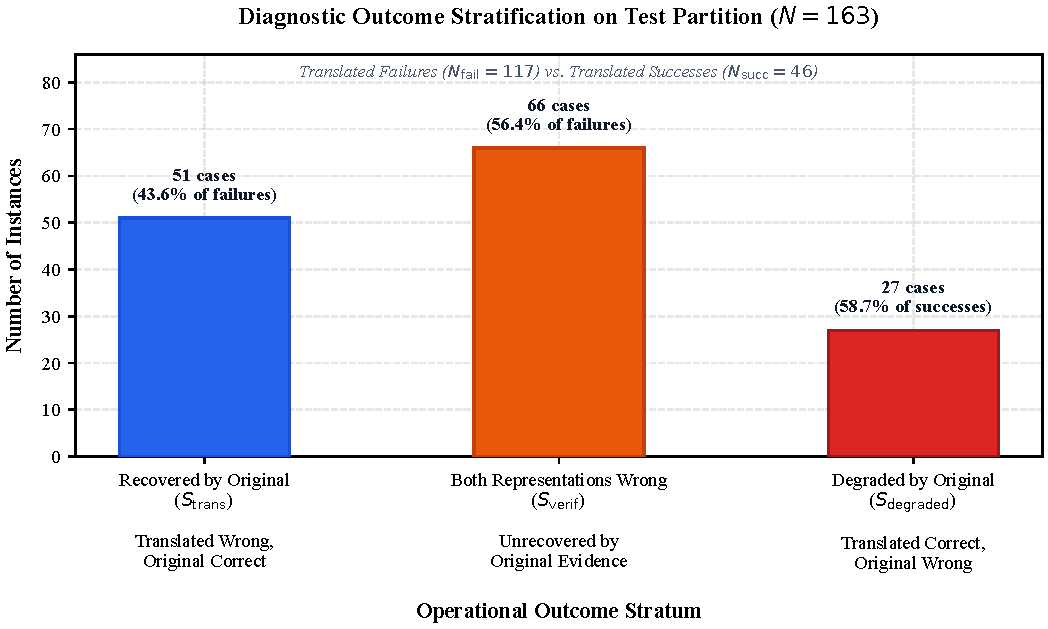
\includegraphics[width=\columnwidth]{figures/final/fig4_error_attribution_breakdown.pdf}
\caption{Decomposition of the 117 translation failures ($N=163$) into recoverable ($S_{\text{trans}}=51$) and unrecoverable ($S_{\text{verif}}=66$) outcomes, alongside degraded cases ($S_{\text{degraded}}=27$).}
\label{fig:fig4_attribution}
\end{figure}

\paragraph{Latency and Compute Profile.}
Table~\ref{tab:main_results} and the canonical latency audit record end-to-end inference latencies measured on an 8-thread CPU environment. The translated-evidence pipeline (\emph{No-Check}) requires a mean of $3,650.4$\,ms per query (comprising $1,688.2$\,ms for MT translation and $1,962.2$\,ms for verifier forward scoring). Direct Multilingual verification on Hindi evidence averages $11,295.6$\,ms per query due to expanded subword tokenization sequence lengths on non-Latin scripts. Unconditional dual verification (\emph{Always-Check}) requires both passes, averaging $14,945.9$\,ms per query. By triggering dual verification on only 7.98\% of instances, \emph{Selective-Check} ($\tau^*=0.650$) achieves a mean end-to-end latency of $4,613.8$\,ms---saving 69.1\% latency relative to Always-Check and 59.2\% relative to Direct Multilingual. However, because its accuracy matches No-Check, this computational saving does not translate into improved veracity verification.
